%------------------------------------------------
\section{Магнетрон}

%------------------------------------------------

\begin{frame}
	\frametitle{Магнетрон}
	\par Магнетрон представляет собой вакуумную лампу, которая работает как самовозбуждающийся микроволновый генератор. Используются скрещенные элестрическое и магнитное поле для получения высокой выходной мощности, необходимой в радиолокационном оборудовании.
	
	\begin{figure}
		\centering
		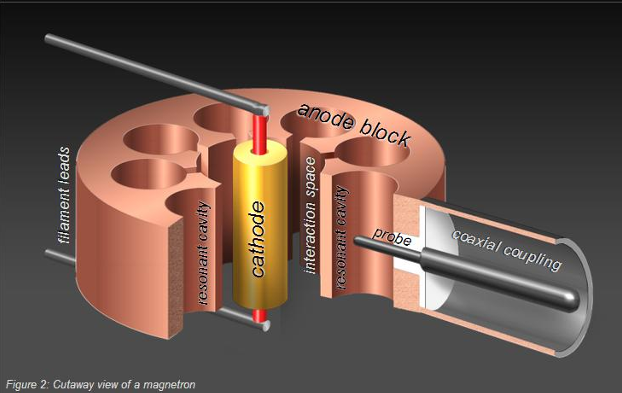
\includegraphics[width=0.4\linewidth]{images/magnetron}
		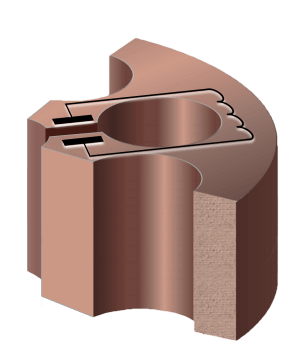
\includegraphics[width=0.2\linewidth]{images/resonator}

	\end{figure}
	
	
\end{frame}

\begin{frame}
	
	\par Анод магнетрона выполнен в виде цилиндрического цельного медного блока. Катод и нить накала расположены в центре трубки и поддерживаются выводами нити накала.
	
	\begin{figure}
		\centering
		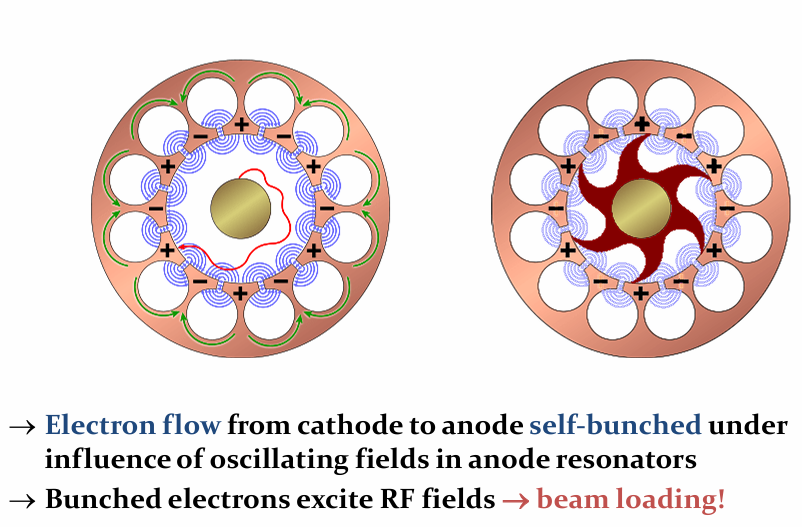
\includegraphics[width=0.60\linewidth]{images/magnetron_loading}
	\end{figure}
	
	
\end{frame}

\begin{frame}
	\begin{figure}
		\centering
		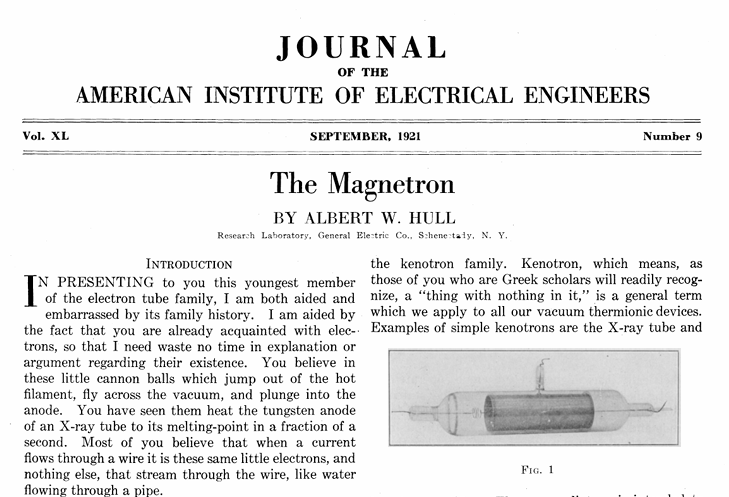
\includegraphics[width=0.65\linewidth]{images/magnetron_history}
	\end{figure}
\end{frame}

\begin{frame}
	\frametitle{Благодарность}
	\begin{center}
		Спасибо за внимание!
	\end{center}
	
\end{frame}
